\section{Zielsetzung}
\label{sec:Zielsetzung}

    In diesem Versuch wird die Ablenkung eines Elektronenstrahls einmal in einem elektrischen Feld und einmal in einem magnetischen Feld untersucht. Dabei wird 
    die spezifische Ladung $\frac{e_0}{m_0}$ eines Elektrons errechnet und das Magnetfeld der Erde am Experimentierort bestimmt. 

\section{Theorie}
\label{sec:Theorie}

Zur Erzeugung eines Elektronenstrahls kann eine Kathodenstrahlröhre, welche auch unter dem Namen Braun'sche Röhre bekannt ist, genutzt werden. Um Wechselwirkungen 
der Elektronen mit Luftmolekülen zu vermeiden, werden alle Teile des Experimentes in einem Hochvakuum durchgeführt. In üblichen Kathodenstrahlröhren herrscht ein Druck von 
etwa $\SI{e-6}{\milli\bar}$. 

\subsection{Kathodenstrahlröhre}

    In einer Kathodenstrahlröhre werden Elektronen mit einer sogenannten Elektronenkanone erzeugt. Dort werden mittels Glühemission Elektronen aus einer
    Kathode, welche eine Oberfläche aus Material mit niedriger Elektronenaustrittsarbeit hat, gelöst. Die Kathode ist von einem Wehnelt-Zylinder umgeben.
    Dies ist ein zylindrischer Hohlkörper an dem ein zur Kathode negatives Potential anliegt. Somit wird die Intensität des Elektronenstrahls gesteuert. 
    Die dritte anliegende Spannung ist die Beschleunigungsspannung $U_{\text{B}}$. Diese gibt den Elektronen Energie, sodass sie die Geschwindigkeit
    \begin{equation} \label{eqn:v_z}
        \frac{m_0 v_{\text{z}}^2}{2} = e_0 \cdot U_{\text{B}}
    \end{equation}
    haben, welche sich aus dem Energiesatz berechnen lässt. Hier beschreibt $e_0$ die Elementarladung, $m_0$ die Elektronenmasse und $v_{\text{z}}$ die 
    Geschwindigkeit der Elektronen, wobei $v_{\text{z}} \ll \symup{c} $ gelten muss. Diese Schaltung ist auch in der \autoref{fig:querschnitt_kathodenstrahlroehre}
    zu sehen.\\

    \begin{figure}[H]
        \centering
        \includegraphics[width=0.8\textwidth]{bilder/querschnitt_kathodenstrahlröhre.png}
        \caption{Der Querschnitt einer Kathodenstrahlröhre und die Beschaltung ihrer Elektronenkanone \cite{anleitung501}.}
        \label{fig:querschnitt_kathodenstrahlroehre}
    \end{figure}

    \noindent Die ausgelösten und beschleunigten Elektronen werden anschließend mit einer elektronischen Linse gebündelt. Dies geschieht durch inhomogene E-Felder, 
    welche sich am Stirnende der Elektroden aufbauen. Dementsprechend ist die Brechkraft dieser elektronischen Linse mit der Spannung $U_{\text{c}}$ einstellbar.\\
    Der Elektronenstrahl fällt auf einen auf der Innenseite aufgedampften Leuchtschirm. Dort regen die Elektronen die Aktivatorzentren zur Emission von
    Lichtquanten an. Damit sich der Leuchtschirm nicht negativ auflädt ist er elektrisch leitend mit der Beschleunigungselektrode verbunden. \\
    Nach dem Austreten der Elektronen aus der Elektronenkanone durchlaufen diese das Ablenksystem, welches aus zwei senkrecht zueinanderstehenden
    Plattenkondensatoren besteht. Wird dort eine Spannung angelegt, so werden die Elektronen abhängig von der Feldstärke des im Plattenkondensator entstehendem 
    elektrischen Feld und ihrer Geschwindigkeit weit abgelenkt. 

\subsection{Ablenkung eines Elektronenstrahls im elektrischen Feld}

    Liegt an einem Plattenkondensator eine Spannung $U_{\text{d}}$ an, so bildet sich in ihm ein nahezu homogenes elektrisches Feld mit der Feldstärke
    \begin{equation*}
        E = \frac{U_{\text{d}}}{d}, 
    \end{equation*}
    wobei $d$ für den Plattenabstand steht. Befindet sich eine Ladung in diesem Feld, so wirkt auf sie die Kraft
    \begin{equation*}
        |\vec{F}| = e_0 \cdot \frac{U_{\text{d}}}{d}.
    \end{equation*}
    Die Richtung der Kraft ist parallel oder antiparallel zu den Feldlinien. Da die Kraft nur im elektrischen Feld auf die Ladung ausgeübt wird, kann die Geschwindigkeit, 
    die die Ladung nach Durchlauf des Plattenkondensators in y-Richtung hat, angegeben werden mit  
    \begin{equation*}
        v_{\text{y}} = a_{\text{y}} \cdot \increment t = \frac{F}{m_0} \increment t. 
    \end{equation*}
    Dazu wird genutzt, dass $v = a \cdot t$ und $F = m \cdot a$ ist. Mit der Geschwindigkeit in z-Richtung, welche durch die Beschleunigungsspannung gegeben ist, 
    kann die Durchlaufzeit $\increment t$ angegeben werden als $\increment t = \frac{p}{v_{\text{z}}}$. Somit gilt für die Geschwindigkeit in y-Richtung:
    \begin{equation*}
        v_{\text{y}} = \frac{e_0}{m_0} \frac{U_{\text{d}}}{d} \frac{p}{v_{\text{z}}}
    \end{equation*}
    
    \begin{figure}
        \centering
        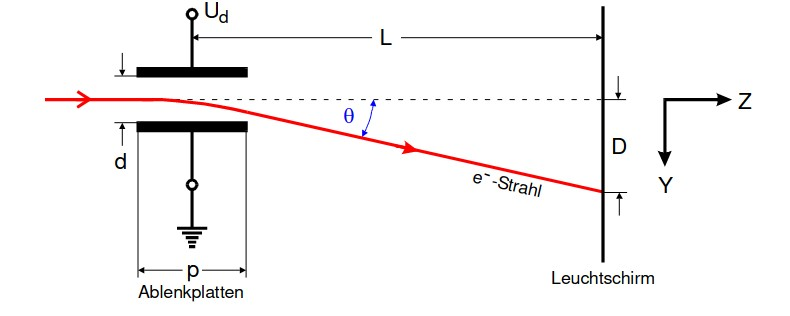
\includegraphics[width=\textwidth]{bilder/strahlablenkung_efeld.jpg}
        \caption{Die Strahlablenkung in der Kathodenstrahlröhre \cite{anleitung501}.}
        \label{fig:strahlablenkung_efeld}
    \end{figure}

    \noindent In der \autoref{fig:strahlablenkung_efeld} ist die beschriebene Ablenkung mit allen wichtigen Größen eingezeichnet. Es ist zu beachten, dass die Auslenkung
    des Elektronenstrahl direkt beim Eintritt in den Kondensator beginnt und nicht erst in der Mitte des Kondensators. Da sich das Elektron außerhalb des E-Feldes 
    geradlinig bewegt, kann mithilfe der \autoref{fig:strahlablenkung_efeld} für den Winkel der Richtungsänderung der Term 
    \begin{equation*}
        \theta \approxeq \frac{v_{\text{y}}}{v_{\text{z}}} = \frac{e_0}{m_0} \frac{U_{\text{d}}}{d} \frac{p}{v_{\text{z}}^2}
    \end{equation*}
    angegeben werden. Es wird die Kleinwinkelnäherung angenommen. Die messbare Verschiebung des angezeigen Punktes auf dem Leuchtschirm $D$ wird unter Benutzung der Kleinwinkelnäherung
    berechnet über
    \begin{equation}
        \label{eqn:pL_2d}
        D = L \cdot \theta = \frac{e_0}{m_0} L \frac{U_{\text{d}}}{d} \frac{p}{v_{\text{z}}^2} = \frac{p}{2d} L \frac{U_{\text{d}}}{U_{\text{B}}}. 
    \end{equation}
    Bei der letzten Umformung wird für $v_{\text{z}}$ die Relation aus Gleichung \eqref{eqn:v_z} eingesetzt. \\

    \noindent Aus den Formeln ist zu erkennen, dass für eine hohe Ablenkempfindlichkeit ein langer Ablenkkondensator $p$, ein langer Strahlenweg $L$ und eine geringe Beschleunigungsspannung 
    genutzt werden muss. Da die Flugzeit $\increment t$ immer klein gegenüber der Periodendauer von $U_{\text{d}}$ sein muss, können so nur niederfrequente Wechselspannungen gemessen
    werden. Um hochfrequente Wechselspannungen zu untersuchen, wird eine Kathodenstrahlröhre mit kurzem Ablenkkondensator $p$ und großer Beschleunigungsspannung benötigt.

\subsection{Prinzip eines Kathodenstrahl-Oszillographen}

    Eine Kathodenstrahlröhre kann auch als Kathodenstrahl-Oszillograph benutzt werden, indem die zu untersuchende Spannung auf die vertikal ablenkenden Platten und eine Sägezahnspannung 
    auf die horizontal ablenkenden Platten angelegt wird. Die Sägezahnspannung steigt linear an und fällt beim Erreichen ihres Maximalwertes schlagartig wieder auf die Null. 
    Damit sorgt sie dafür, dass der Elektronenstrahl gleichmäßig über den Leuchtschirm fährt und beim Erreichen des Endes des Leuchtschirms springt der Elektronenstrahl wieder an
    den Anfang des Leuchtschirms. Um ein stehendes Bild auf dem Schirm zu sehen, muss für die Frequenzen der folgende Zusammenhang gelten
    \begin{equation}\label{eqn:frequenzen}
        n \cdot \nu_{\text{Sä}} = m \cdot \nu_{\text{We}},
    \end{equation}
    wobei $n,m \in \symbb{N}$ sind. Für $n=1, m=2$ bedeutet das, dass auf dem Schirm zwei Periodendauern der Wechselspannung zu sehen sind.

\subsection{Ablenkung eines Elektronenstrahls im homogenen Magnetfeld}

    In einem homogenen Magnetfeld wirkt auf bewegte Ladungen die sogenannte Lorentz-Kraft 
    \begin{equation} \label{eqn:lorentzforce}
        \vec{F} = q\cdot \vec{v} \times \vec{B}.
    \end{equation}
    Kommt ein Elektron mit einer Geschwindigkeit in z-Richtung in ein homogenes Magnetfeld, welches in x-Richtung ausgerichtet ist, so erfährt es eine Kraft in y-Richtung, 
    \begin{equation*}
        F_{\text{L, y}} = e_0 m_0 B.
    \end{equation*}
    Die Geschwindigkeit in y-Richtung, welche aus der Kraft resultiert, überlagert sich mit der Geschwindigkeit in z-Richtung, sodass das Elektron auf eine gekrümmte Bahn in der 
    xy-Ebene gezogen wird. Eine Eigenschaft des Kreuzproduktes aus der Formel \eqref{eqn:lorentzforce} ist, dass die Kraft senkrecht auf dem Wegelement steht,
    \begin{equation*}
        \vec{F} \cdot \vec{\symup{d}s} = 0.
    \end{equation*}
    Hieraus folgt, dass sich die potentielle Energie des Elektrons nicht ändert. Da Energieerhaltung gilt, muss somit auch kinetische Energie $E_{\text{kin}} = \frac{1}{2} m_0 v^2$
    konstant bleiben und damit bleibt als einzig veränderbare Variable $|\vec{v}|$. Außerhalb des Magnetfeldes ist die Geschwindigkeit $\vec{v} = v_{\text{z}} \vec{\symup{e}_{\text{z}}}$, sodass 
    \begin{equation*}
        |\vec{v}| = v_{\text{z}}
    \end{equation*}
    für alle Bahnpunkte gilt. Durch Gleichsetzen von Lorentzkraft und Zentripetalkraft kann der momentane Krümmungsradius $r$ ermittelt werden:
    \begin{align} \label{eqn:r}
        e_0 m_0 B &= \frac{m_0 v_{\text{z}}}{r} &\implies r &= \frac{m_0 v_{\text{z}}}{e_0 B}
    \end{align}
    Es ist auffällig, dass der Radius sich nur aus kostanten Werten zusammensetzt, sodass sich das Elektron auf einer Kreisbahn bewegen muss. \\

    \begin{figure} 
        \centering
        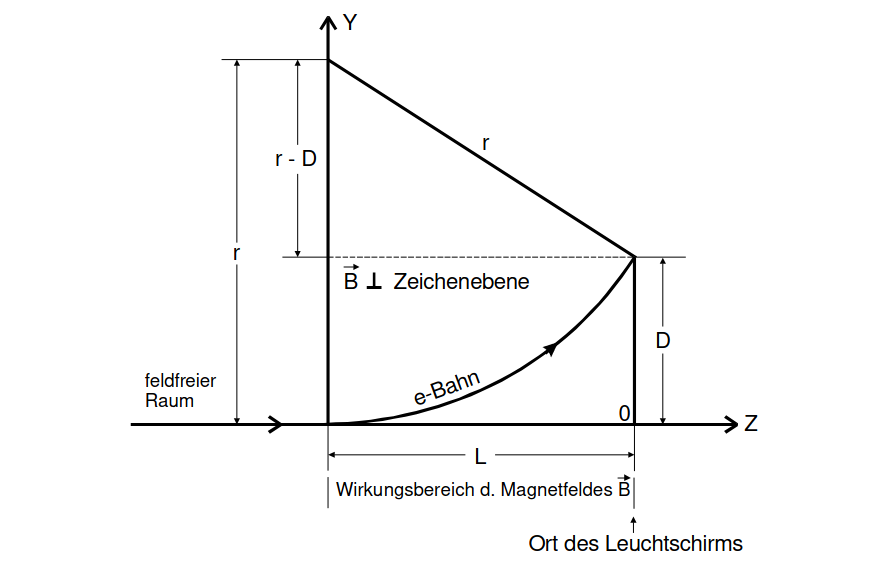
\includegraphics[width=\textwidth]{bilder/zeichnung_magnetfeld.png}
        \caption{Skizze zur Bestimmung der Beziehungen bei der Ablenkung im B-Feld \cite{anleitung502}.}
        \label{fig:skizze_bfeld}
    \end{figure}

    \noindent In der Kathodenstrahlröhre bekommen die Elektronen die Geschwindigkeit 
    \begin{equation*}
        v_{\text{z}} = \sqrt{\frac{2 U_{\text{B}}e_0}{m_0}},
    \end{equation*}
    wobei diese aus der Gleichung \eqref{eqn:v_z} durch Umstellen ermittelt wird. Auf dem Leuchtschirm ist der Abstand vom Nullpunkt $D$ zu ermitteln.
    Ist $L$, wie in der \autoref{fig:skizze_bfeld} zu sehen der Wirkungsbereich des Magnetfeldes, so gilt der Zusammenhang
    \begin{align*}
        L^2 + (r - D)^2 &= r^2  &\implies r &= \frac{L^2 + D^2}{2D}.
    \end{align*}
    Durch Einsetzen der Zusammenhänge \eqref{eqn:r} und \eqref{eqn:v_z} lässt sich ein Ausdruck für die spezifische Ladung aufstellen:
    \begin{equation}\label{eq:e0_m0}
        \frac{D}{L^2 + D^2} = \frac{1}{\sqrt{8 U_{\text{B}}}} \cdot \sqrt{\frac{\symup{e_0}}{\symup{m_0}}} \cdot B.
    \end{equation}